\documentclass[11pt,a4paper]{article}
\usepackage{graphicx}
\usepackage{float}
\usepackage{natbib}
\usepackage{amsmath, amsthm, amssymb}
\usepackage{amsfonts}
\usepackage{makeidx}
\usepackage{lmodern}
\usepackage{grffile}
\graphicspath{ {figures/} }
\usepackage{array}
\usepackage{tocloft}
\usepackage{mathrsfs}
\usepackage[final]{pdfpages}
\usepackage{fancyhdr}
\usepackage{xcolor}
\usepackage[colorlinks = true,
            linkcolor = blue,
            urlcolor  = blue,
            citecolor = blue,
            anchorcolor = blue]{hyperref}

\usepackage[left=2cm,right=2cm,top=2cm,bottom=2cm]{geometry}
\linespread{1}

\setlength{\headheight}{14pt} 
\title{Professional Development Plan}
\author{Pierre Le Roux}
\pagestyle{fancy}
\lhead{Pierre Le Roux}
\chead{Professional Development Plan}
\rhead{u13112262}

\begin{document}

	\begin{titlepage}
		\noindent\makebox[\linewidth]{\rule{\paperwidth}{0.4pt}}
		
		\centering
		\vspace*{1cm}
		{\scshape\LARGE Professional Development Plan \par}
		\vspace{1,5cm}		
		{ by \par}
		\vspace{1,5cm}
		{\scshape\LARGE Pierre Le Roux \\
						u13112262\par}
		\vspace{1,5cm}	
		{ for \par}
		\vspace{1,5cm}
		{\scshape\LARGE IPI 410}
						
	%Insert Figure
		\vspace{2,5cm}
		
\includegraphics[width=\textwidth]{Extra/Tuks_Logo.jpg}
		

	% Bottom of the page
		\vfill						
		{\large May 16, 2016\par}
		
		\vspace*{1cm}	
		\noindent\makebox[\linewidth]{\rule{\paperwidth}{0.4pt}}
	\end{titlepage}
	
	\pagebreak
	
	\pagenumbering{arabic}
	\setcounter{page}{1}
	
	\section{Purpose}
		The purpose of this plan is to ensure that all requirements in terms of ECSA outcomes are met, in the minimum amount of time of five years, by future candidate engineer Mr Pierre Le Roux (13112262) which will be referred to in this paper as FCE.
		The plan will cover the following:
		
		\begin{enumerate}
		\item	Registering at ECSA as a Professional Industrial Engineer
		
		\item	Completing one five year cycle of Continuous Professional Development (CPD)
		\end{enumerate}
		
		This plan isn't perfect and as circumstances change the plan will be rescheduled accordingly while still ensure that the FCE achieves said outcomes.
		
	\section{Directions}
		During the FCE's studies automation, simulation, operations research, processes and production automation peaks his interest. 
		The FCE's final year project , Improving FlySafair's Crew Scheduling, is an operations research project which combines programming, heuristics and modelling to create a more automated system the insures to generate a more optimal schedule for FlySafair.
		
	
	\section{Commitments}
		The FCE's has not commitments to a third party in terms of completing his B.Ing. degree.
		While it is fortunate that the FCE doesn't have any contractual requirement in terms of employment, but on the other hand the FCE will need to find employment to ensure he can complete the requirements in terms of the eleven ECSA outcomes and completing activities for CPD credits - Developmental, work-based and individual.
	
	\section{CDP To Achieve Professional Registration}
		If the FCE passes all his module this year he will graduate at the end of 2016.
		The FCE hopes that FlySafair would provide work for him based on the results of his final year project.
		Concerning the FCE's interests the following directions, but not limited to, are available:
		
		\begin{enumerate}
		\item	\textbf{Automation and Control} in decision support mechanisms
		
		\item	\textbf{Operations Research} in logistics
		
		\item	\textbf{Processes} in service industries
		
		\item	\textbf{Robotics and Production} in manufacturing industries
		
		\end{enumerate}
		
		Development in any of the above field is acceptable according to CITE(ECSA 2013a) as it is specific to the industrial engineering field. With FlySafair \textbf{Automation and Control} and \textbf{Operations Research} will be developed over a period of 36 months to comply with outcomes as stated in CITE(ECSA 2012).
		
	\subsection{ECSA's Eleven Competency Standards}
		In figure \ref{fig: ECSA}, ECSA's eleven outcomes are summaries as stated in R-08-PE. 
		Theses consists of five main groups:
		
		\begin{itemize}
		
		\item[]	\textbf{Group A:} Knowledge-based Engineering Problem Solving (Outcomes 1, 2, 3)
			

		\item[]	\textbf{Group B:} Managing Engineering Activities (Outcomes 4, 5)

		\item[]	\textbf{Group C:} Risk and Impact Mitigation (Outcomes 6, 7)

		\item[]	\textbf{Group D:} Exercising Judgement and Taking Responsibility (Outcomes 8, 9, 10)

		\item[]	\textbf{Group E:} Developing Own Competency (Outcome 11)
				
		\end{itemize}

		\begin{figure}[H]
		\centering
		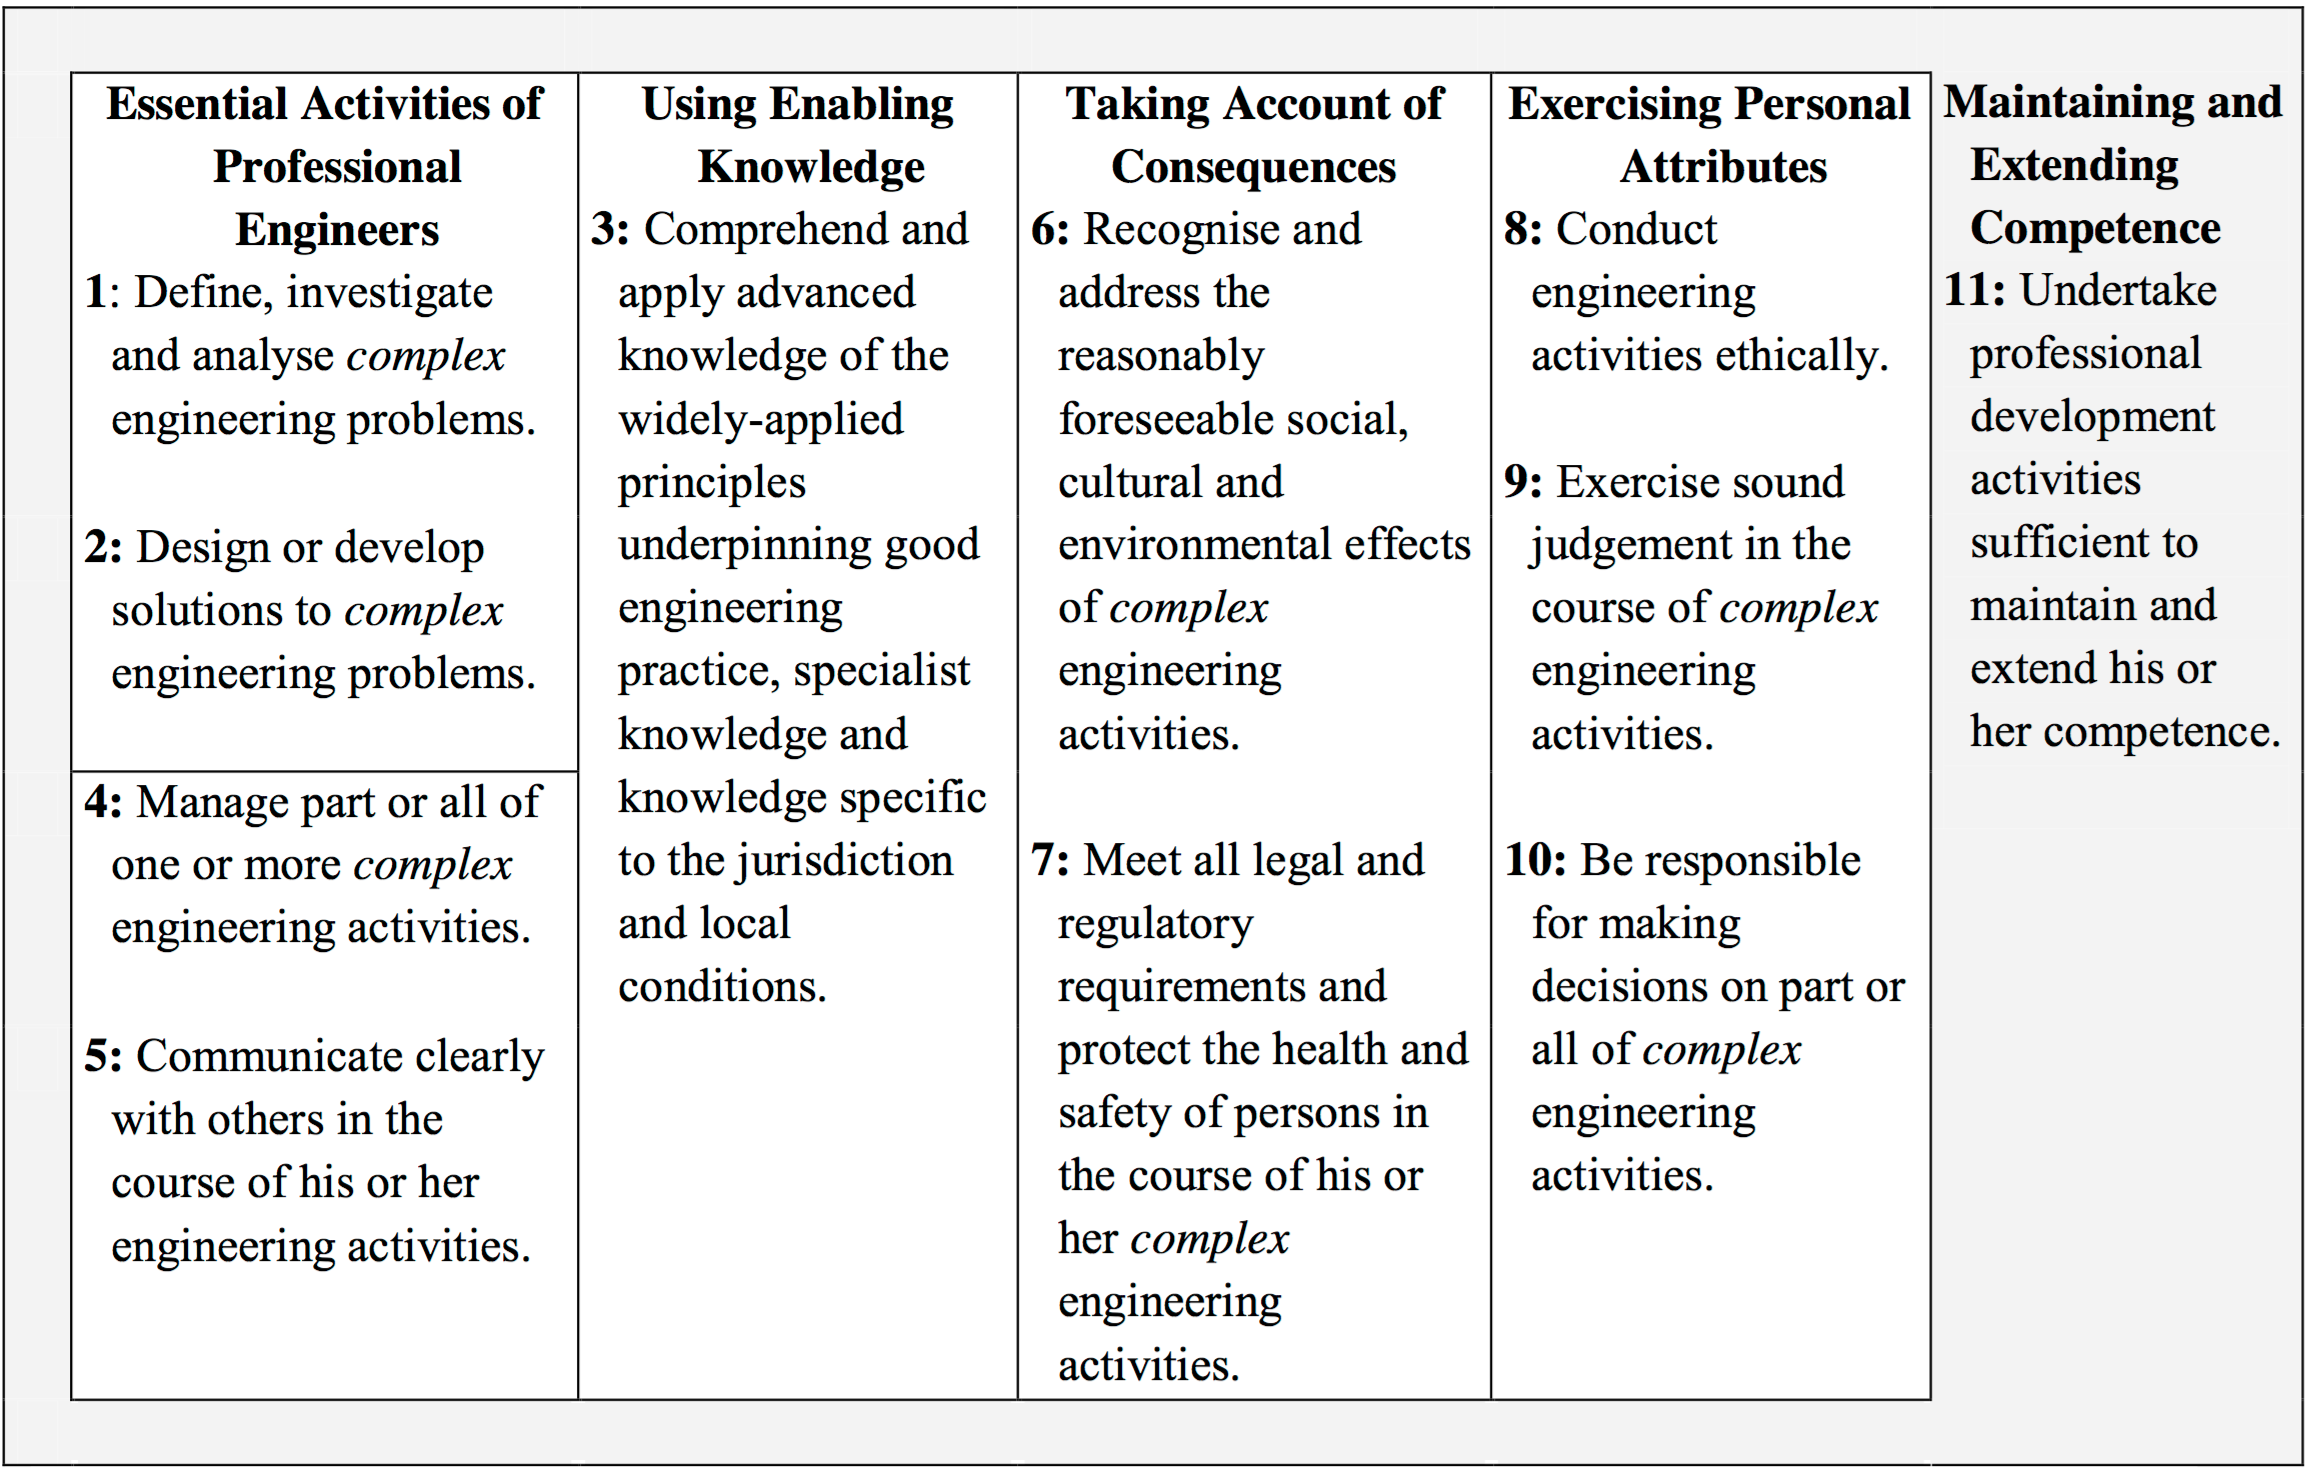
\includegraphics[width=\textwidth]{Extra/ECSA_Outcomes.png}
		\caption{Nested ECSA Outcomes for Registration as a Professional Engineer}\label{fig: ECSA}
		\end{figure}
		
		https://www.ecsa.co.za/RegisterDocuments/R-02-PE.pdf
		
		$https://www.ecsa.co.za/ECSADocuments/ECSA%20Documents/Documents/R-05-IND-PE.pdf$
		
		$https://www.ecsa.co.za/ECSADocuments/ECSA%20Documents/Documents/R-08-PE.pdf$
		
		https://www.ecsa.co.za/maintainregistration/MaintainReg/CPD_Policy.pdf
		
		https://www.ecsa.co.za/regulation/RegulationDocs/2014_Code_of_Conduct.pdf
		
		https://www.saiie.co.za/cms/category/53-approved-courses
		
		https://www.saiie.co.za/cms/section/8-
	
	\section{Full CPD Cycle as a Registered Professional Engineer}
	
	\section{What are the risks?}
				

\end{document}
